\section{Auswertung}

% -------------Magnetfeld------------
\subsection{Magnetfeldmessung}
Zu Beginn des Experiments wird das Magnetfeld in Abhängigkeit des Spulenstroms bestimmt (\ref{tab:Br}).
Zwischen den beiden Größen besteht ein linearer Zusammenhang, daher lässt sich die Kurve durch eine Ausgleichsgerade annähern.
% Data 2
\begin{table}[H]
    \centering
    \begin{tabular}{c c}
        \toprule
        $I_{Spule} \;/\;$A & $B\;/\;$mT\\
        \midrule
        0,0                 &0,0\\
        0,5                 &132,4\\
        1,0                 &270,0\\
        1,5                 &413,7\\
        2,0                 &556,4\\  
        2,5                 &698,3\\
        3,0                 &828,3\\
        3,5                 &956,0\\
        4,0                 &1063,9\\
        4,5                 &1145,2\\
        5,0                 &1204,5\\
        \bottomrule
    \end{tabular}
    \caption{Magnetfeldmessung (reihe)}
    \label{tab:Br}
\end{table}
% Plot 2
\begin{figure}[H]
    \centering
    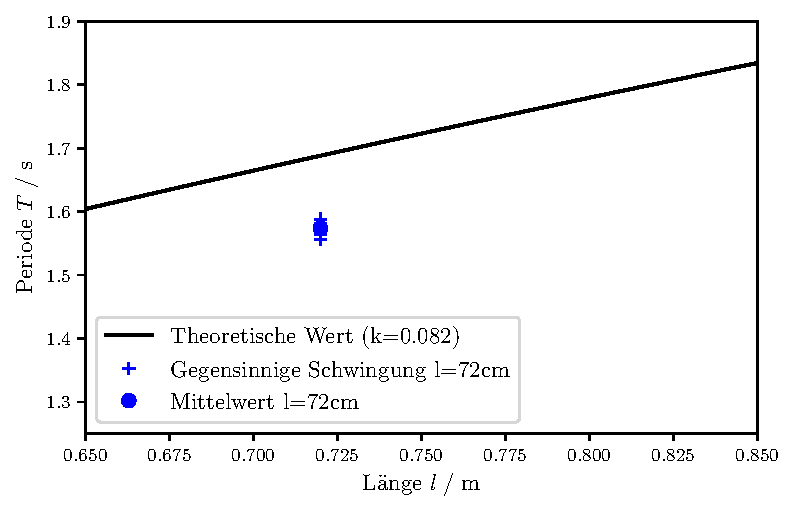
\includegraphics{build/plot2.pdf}
    \caption{B-Feld Messung}
    \label{fig:Br}
\end{figure}
Mit der Ausgleichsgeraden
\begin{align*}
    y &= mx + b\\
    m &= \SI{251\pm 8}{\milli \tesla \per \ampere} \\  
    b &= \SI{32\pm 24}{\milli \tesla}\\
\end{align*}
Aus der Umkerfunktion dieser Ausgleichsrechnung lässt sich in den folgenden Berechnungen das B-Feld aus dem angelegten Spulenstrom bestimmen.

\subsection{Die Bestimmung der mikroskopischen Parameter}
\label{subsubsec:mikro_Param}
Über eine Ausgleichsgerade lässt sich die Anzahl der Ladungsträger pro Volumen sowohl in Abhängigkeit vom B-Feld (bei konstantem $I_{quer}$) als auch in Abhängigkeit vom Querstrom (bei konstantem $B$) bestimmen.
Die folgenden Rechnungen werden für jedes Material somit einmal mit dem aus dem B-Feld berechneten und einmal mit dem aus dem Querstrom berechneten Wert durchgeführt.
Die Anzahl der Ladungsträger bestimmt sich mit
\begin{align*}
    n &= -\frac{1}{e_0 U_H d}\cdot B\cdot I_q \\
    y &= \;\;\; \; \; \; \; \;   m \;  \; \cdot \; \; \; x \; \; \; \; \; \; \; \; \; +b\\
\end{align*}
Weiterhin lässt sich mit den so errechneten Werten für n der Energie Parameter $E_F$ berechnen.
\begin{align*}
    E_F &= \frac{h^2}{2 m_0}\cdot \left(\frac{3}{8\pi}\cdot n \right)^{\frac{2}{3}} \\
    \Delta E_F &= \left( \frac{9 h^2  \left(\Delta n\right)^2}{192 \pi^2 m_0} \cdot \left( \frac{9}{64\pi^2} \Delta n^2\right)^{-\frac{2}{3}}  \right)
\end{align*}
Über $E_F$ lässt sich der nächste Parameter, die Totalgeschwindigkeit $|\bar{v}|$, berechnen.
\begin{align*}
    |\bar{v}| &= \left(\frac{2 E_F}{m_0}\right)^{\frac{1}{2}} \\
    \Delta |\bar{v}| &= \frac{1}{2} \left(\frac{2 \Delta E_F}{m_0}\right)^{-\frac{1}{2}}
\end{align*}
Außerdem lässt sich aus n und der zuvor berechneten spezifischen Leitfähigkeit $\rho$ die mittlere Flugzeit $\bar{\tau}$ berechnen.
\begin{align*}
    \bar{\tau} &= 2 \frac{m_0}{e_0^2} \cdot \frac{1}{n \rho} \\
    \Delta \bar{\tau} &= \sqrt{ \left( -2 \frac{m_0}{e_0^2} \cdot \frac{1}{n^2 \rho} \cdot \Delta n \right)^2 + \left( -2 \frac{m_0}{e_0^2} \cdot \frac{1}{n \rho^2} \cdot \Delta \rho \right)^2 }
\end{align*}
Aus der mitlleren Flugzeit $\bar{\tau}$ kann dann noch die mittlere freie Weglänge $\bar{l}$ bestimmt werden.
\begin{align*}
    \bar{l} &= \bar{\tau} \cdot |\bar{v}| \\
    \Delta \bar{l} &= \sqrt{\left(|\bar{v}|\cdot\Delta\bar{\tau}\right)^2+\left(\bar{\tau}\cdot|\bar{v}|\right)^2}
\end{align*}
Nun muss noch die Beweglichkeit der Ladungsträger $\mu$ über das äußere elektrische Feld $\vec{E}$ und die Driftgeschwindigkeit $\vec{\bar{v}}_d$ bestimmt werdenbestimmt werden
\begin{align*}
    \vec{\bar{v}}_d &= -\frac{n \cdot e_0}{j} \\
    \Delta \vec{\bar{v}}_d &= - \frac{e_0}{j}\Delta{n}\\
    \mu &= 2 \frac{m_0 j}{e_0^2} \cdot \frac{1}{n  \bar{\tau}}\\
    \Delta \bar{\mu} &= \sqrt{
        \left( -2 \frac{m_0 j}{e_0^2} \cdot \frac{1}{n^2 \bar{\tau}} \cdot \Delta n \right)^2 
        + \left( -2 \frac{m_0 j}{e_0^2} \cdot \frac{1}{n \bar{\tau^2}} \cdot \Delta \bar{\tau} \right)^2 
        }\\
\end{align*}

%|||||||||||||||||||||||||||||||||||||||||||||||||||||||||||||||||||||||||||||||||||||||||||||||||||||||||||||||||


% --------KUPFER
\subsection{Kupfer}
\subsubsection{Geometrische Messungen und Wiederstand}
Die Dicke des Kupferblatts konnte auf der Apparatur abgelesen werden.
Die Länge des Kupferdrahts konnte auch abgelesen werden, der Wiederstand wurde jedoch gemessen.
\begin{align*}
    d_{Cu} &= \SI{18}{\micro \meter} \\
    l_{Cu} &= \SI{137}{\centi \meter}\\
    R_{Cu} &= \SI{2,734}{\ohm}\\
    r_{Cu} &= \frac{1}{2}\cdot \SI{0,218}{\milli \meter}
\end{align*}
Daraus lässt sich die spezifische Leitfähigkeit des Materials berechnen.
\begin{align*}
    \rho_{Cu} &= R_{Cu}\cdot \frac{\pi r_{Cu}^2}{l_{Cu}}\\
    \rho_{Cu} &= \SI{0,074\pm0,007}{\micro \ohm \meter}\\
    \rho_{Cu,literatur} &= \SI{0,018}{\micro \ohm \meter} %https://oerttel.net/data/documents/Leitfaehigkeit.pdf
\end{align*}
\subsubsection{Hall Spannung bei konstantem B-Feld}
Um die Abhängigkeit der Hall Spannung vom anliegenden Querstrom $I_q$ festzustellen wurde der Spulenstrom $I_B$ konstant auf 5 Ampere gehalten.
% Data 4
\begin{table}[H]
    \centering
    \begin{tabular}{c c c}
        \toprule
        $I_B \;/\;$A & $U_H\;/\;$mV & $I_q \;/\;$A\\
        \midrule
            5                   & 0,0029&             0\\
            5                   & 0,0005&             1\\
            5                   &-0,0015&             2\\
            5                   &-0,0030&             3\\
            5                   &-0,0044&             4\\
            5                   &-0,0056&             5\\
            5                   &-0,0075&             6\\
            5                   &-0,0088&             7\\
            5                   &-0,0110&             8\\
            5                   &-0,0129&             9\\
            5                   &-0,0140&             10\\
        \bottomrule
    \end{tabular}
    \caption{Hall Spannung für Kupfer- konstantes Magnetfeld}
    \label{tab:Cu_I_b}
\end{table}
% Plot 4
\begin{figure}[H]
    \centering
    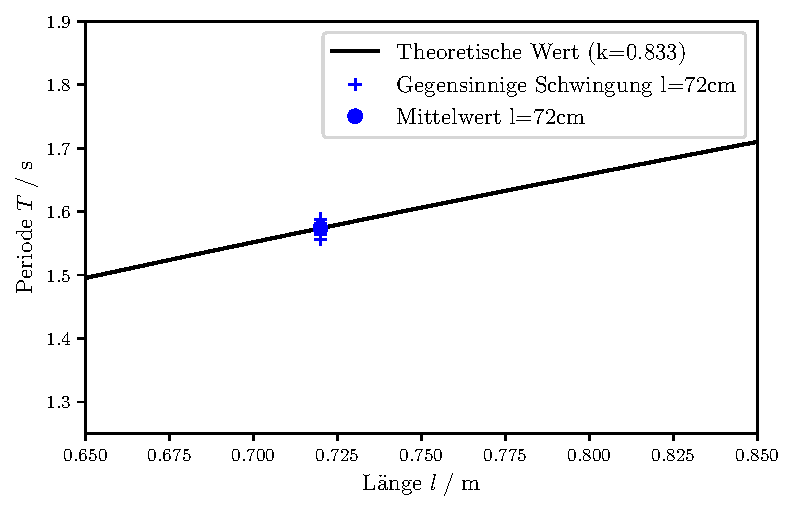
\includegraphics{build/plot4.pdf}
    \caption{Hall Spannung in Abhängigkeit vom Querstrom - Kupfer}
    \label{fig:Cu_I}
\end{figure}
Mit der Ausgleichsgeraden
\begin{align*}
    y &= mx + b\\
    m &= \SI{-164 \pm 4 e-01}{\volt \per \ampere}\\  
    b &= \SI{2,3045 \pm 0,2119}{\volt}\\
\end{align*}

\begin{table}[H]
    \centering
    \begin{tabular}{c c}
        \toprule
        Größe & Wert\\
        \midrule
        $n$   &\SI[per-mode=fraction]{2,71\pm 0,06 e+29}{\per \cubic \metre}\\
        $z$   &\num{3,21\pm 0,07}\\
        $\bar{\tau}$ & \SI{1,454\pm 0,032 e-14}{\second}\\
        $\vec{\bar{v}}_d$ & \SI[per-mode=fraction]{2,30\pm 0,05 e-05}{\metre \per \second} \\
        $\mu$ & \SI[per-mode=fraction]{0,0179}{\coulomb \second \per \kg}\\
        $v_{total}$ & \SI[per-mode=fraction]{2,318\pm 0,017 e+06}{\metre \per \second}\\
        $\bar{l}$ &\SI{3,37\pm 0,05 e-08}{\metre}\\
        \bottomrule
    \end{tabular}
    \caption{Hall Spannung für Kupfer- konstanter Duchflussstrom}
    \label{tab:Cu_I}
\end{table}

\subsubsection{Hall Spannung bei konstantem Querstrom}
Um die Abhängigkeit der Hall Spannung vom äußeren Magnetfeld $B$ festzustellen wurde der Querstrom $I_q$ konstant auf 10 Ampere gehalten.
% Data 3
\begin{table}[H]
    \centering
    \begin{tabular}{c c c}
        \toprule
        $I_{B} \;/\;$A & $U_H\;/\;$mV & $I_{q} \;/\;$A\\
        \midrule
        0                   &0,0081              &10\\
        0,5                 &0,0055              &10\\
        1,0                 &0,0039              &10\\
        1,5                 &0,0012              &10\\
        2,0                 &-0,0008             &10\\
        2,5                 &-0,0025             &10\\
        3,0                 &-0,0048             &10\\
        3,5                 &-0,0068             &10\\
        4,0                 &-0,0086             &10\\
        4,5                 &-0,0097             &10\\
        5,0                 &-0,0110             &10\\
        \bottomrule
    \end{tabular}
    \caption{Hall Spannung für Kupfer- konstanter Duchflussstrom}
    \label{tab:Cu_B_b}
\end{table}
% Plot 3
\begin{figure}[H]
    \centering
    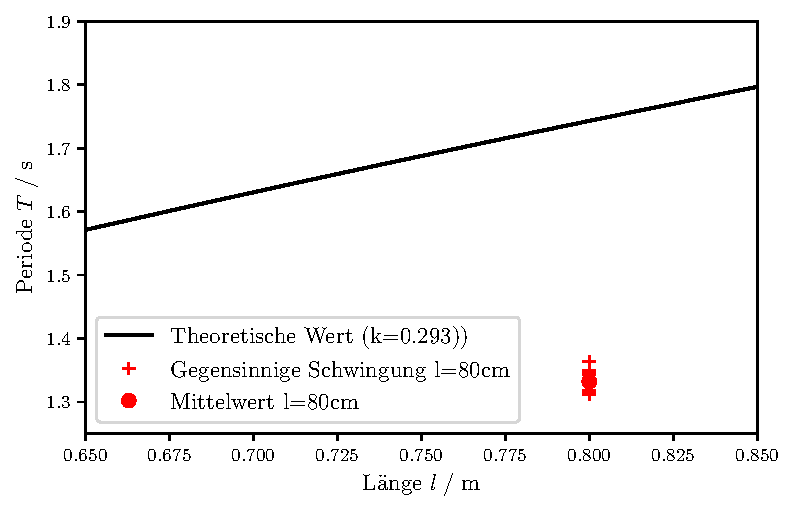
\includegraphics{build/plot3.pdf}
    \caption{Hall Spannung in Abhängigkeit vom Magnetfeld - Kupfer}
    \label{fig:Cu_B}
\end{figure}
Mit der Ausgleichsgeraden
\begin{align*}
    y &= a \cdot x + b\\
    a &=  \SI{-15,4 \pm 0,5 }{\square \meter \per \second}\\
    b &=  \SI{7,9\pm0,4}{\volt}\\
\end{align*}
\begin{table}[H]
    \centering
    \begin{tabular}{c c}
        \toprule
        Größe & Wert\\
        \midrule
        $n$   &\SI[per-mode=fraction]{2,24\pm 0,06 e+29}{\per \cubic \metre}\\
        $z$   &\num{2,65 \pm 0,08}\\
        $\bar{\tau}$ & \SI{1,76\pm 0,05 e-14}{\second}\\
        $\vec{\bar{v}}_d$ & \SI[per-mode=fraction]{2,79\pm 0,08 e-05}{\metre \per \second} \\
        $\mu$ & \SI[per-mode=fraction]{0,018}{\coulomb \second \per \kg}\\
        $v_{total}$ & \SI[per-mode=fraction]{2,175 \pm 0,021 e+06}{\metre \per \second}\\
        $\bar{l}$ &\SI{3,83\pm 0,07 e-08}{\metre}\\
        \bottomrule
    \end{tabular}
    \caption{Hall Spannung für Kupfer- konstanter Duchflussstrom}
    \label{tab:Cu_B}
\end{table}



%|||||||||||||||||||||||||||||||||||||||||||||||||||||||||||||||||||||||||||||||||||||||||||||||||||||||||||||||||


% --------SILBER
\subsection{Silber}
\subsubsection{Geometrische Messungen und Wiederstand}
Die Dicke des Silberblatts konnte nicht gemessen werden, da keine Probe vorlag.
Die Länge des Silberdrahts konnte auf der Apparatur abgelesen werden,der Wiederstand und die Drahtdicke wurde gemessen.
\begin{align*}
    d_{Ag} &= \SI{18}{\micro \meter} \\
    l_{Ag} &= \SI{137}{\centi \meter}\\
    R_{Ag} &= \SI{0.5873}{\ohm}\\
    r_{Ag} &= \frac{1}{2}\cdot \SI{0,218}{\milli \meter}
\end{align*}
Daraus lässt sich die spezifische Leitfähigkeit des Materials berechnen.
\begin{align*}
    \rho_{Ag} &= R_{Ag}\cdot \frac{\pi r_{Ag}^2}{l_{Ag}}\\
    \rho_{Ag} &= \SI{0,0127 \pm 0,0012}{\micro \ohm \meter}\\
    \rho_{Ag,literatur} &= \SI{0,016}{\micro \ohm \meter} %https://oerttel.net/data/doAgments/Leitfaehigkeit.pdf
\end{align*}

\subsubsection{Hall Spannung bei konstantem B-Feld}
Um die Abhängigkeit der Hall Spannung vom anliegenden Querstrom $I_q$ festzustellen wurde der Spulenstrom $I_B$ konstant auf 5 Ampere gehalten.
%data8
\begin{table}[H]
    \centering
    \begin{tabular}{c c c}
        \toprule
        $I_{Spule} \;/\;$A & $U_H\;/\;$mV & $I_{durch} \;/\;$A\\
        \midrule
  5                   &0,0005&              0\\
  5                   &-0,0207&             1\\
  5                   &-0,0394&             2\\
  5                   &-0,0599&             3\\
  5                   &-0,0794&             4\\
  5                   &-0,0991&             5\\
  5                   &-0,1185&             6\\
  5                   &-0,1394&             7\\
  5                   &-0,1602&             8\\
  5                   &-0,1821&             9\\
  5                   &-0,2026&             10\\

       \bottomrule
    \end{tabular}
    \caption{Hall Spannung für Silber- konstantes Magnetfeld}
    \label{tab:Ag_I}
\end{table}
% Plot 8
\begin{figure}[H]
    \centering
    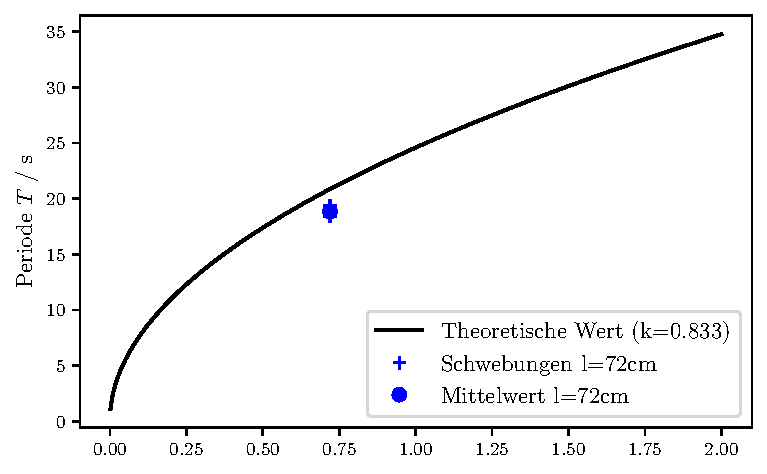
\includegraphics{build/plot8.pdf}
    \caption{Hall Spannung in Abhängigkeit vom Querstrom - Silber}
    \label{fig:Ag_I}
\end{figure}
Mit der Ausgleichsgeraden
\begin{align*}
    y &= mx + b\\
    m &= \SI{-201 \pm 1 e-02}{\volt \per \ampere} \\
    b &= \SI{0,9 \pm 0,6}{\volt}\\
\end{align*}
Mithilfe der Steigung konnten nun die mikroskopischen Parameter berechnet werden.
\begin{table}[H]
    \centering
    \begin{tabular}{c c}
        \toprule
        Größe & Wert\\
        \midrule
        $n$   &\SI[per-mode=fraction]{1,019\pm 0,006 e+26}{\per \cubic \metre}\\
        $z$   &\num{0,001740\pm0,000009}\\
        $\bar{\tau}$ & \SI{4,353\pm 0,024 e-11}{\second}\\
        $\vec{\bar{v}}_d$ & \SI[per-mode=fraction]{0,06124\pm 0,00033}{\metre \per \second} \\
        $\mu$ & \SI[per-mode=fraction]{0,0159}{\coulomb \second \per \kg}\\
        $v_{total}$ & \SI[per-mode=fraction]{1,6729\pm 0,0030 e+05}{\metre \per \second}\\
        $\bar{l}$ &\SI{7,281\pm 0,026 e-06}{\metre}\\
        \bottomrule
    \end{tabular}
    \caption{Hall Spannung für Kupfer- konstanter Duchflussstrom}
    \label{tab:Cu_B}
\end{table}


\subsubsection{Hall Spannung bei konstantem Querstrom}
Um die Abhängigkeit der Hall Spannung vom äußeren Magnetfeld $B$ festzustellen wurde der Querstrom $I_q$ konstant auf 10 Ampere gehalten.
% Data 7
\begin{table}[H]
    \centering
    \begin{tabular}{c c c}
        \toprule
        $I_{Spule} \;/\;$A & $U_H\;/\;$mV & $I_{durch} \;/\;$A\\
        \midrule
            0                   &-0,1707&             10\\
            0,5                 &-0,1740&             10\\
            1,0                 &-0,1777&             10\\
            1,5                 &-0,1809&             10\\
            2,0                 &-0,1850&             10\\
            2,5                 &-0,1885&             10\\
            3,0                 &-0,1909&             10\\
            3,5                 &-0,1945&             10\\
            4,0                 &-0,1970&             10\\
            4,5                 &-0,1990&             10\\
            5,0                 &-0,2002&             10\\
       \bottomrule
    \end{tabular}
    \caption{Hall Spannung für Silber- konstanter Durchflussstrom}
    \label{tab:Ag_I}
\end{table}
% Plot 7
\begin{figure}[H]
    \centering
    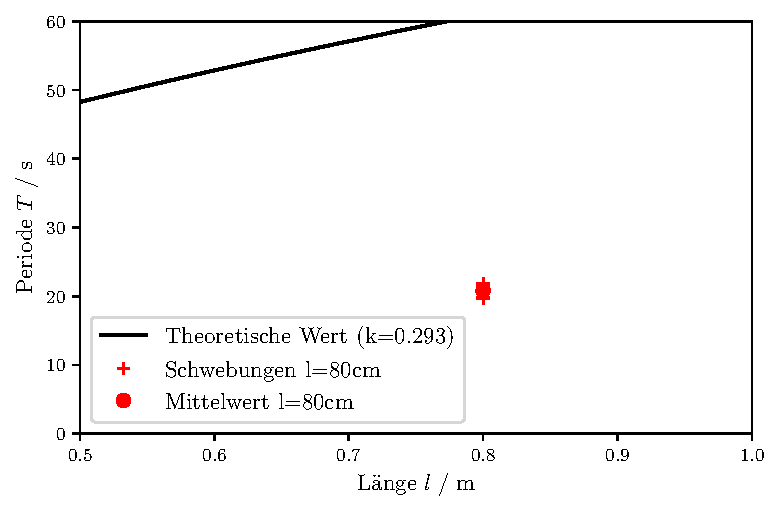
\includegraphics{build/plot7.pdf}
    \caption{Hall Spannung in Abhängigkeit vom Magnetfeld - Silber}
    \label{fig:Ag_B}
\end{figure}
Mit der Ausgleichsgeraden
\begin{align*}
    y &= mx + b\\
    m &= \SI{-24,5 \pm 0,8}{\square \meter \per \second} \\
    b &= \SI{-170,9 \pm 0,6}{\volt} \\ 
\end{align*}
Über die Steigung wurden die mikroskopischen Parameter berechnet.
\begin{table}[H]
    \centering
    \begin{tabular}{c c}
        \toprule
        Größe & Wert\\
        \midrule
        $n$   &\SI[per-mode=fraction]{2,55\pm 0,09 e+28}{\per \cubic \metre}\\
        $z$   &\num{0,435\pm0,016}\\
        $\bar{\tau}$ & \SI{1,74\pm 0,06 e-13}{\second}\\
        $\vec{\bar{v}}_d$ & \SI[per-mode=fraction]{0,000245\pm 0,000009}{\metre \per \second} \\
        $\mu$ & \SI[per-mode=fraction]{0,016}{\coulomb \second \per \kg}\\
        $v_{total}$ & \SI[per-mode=fraction]{1,054\pm 0,013 e+06}{\metre \per \second}\\
        $\bar{l}$ &\SI{1,84\pm 0,04 e-07}{\metre}\\
        \bottomrule
    \end{tabular}
    \caption{Hall Spannung für Kupfer- konstanter Duchflussstrom}
    \label{tab:Cu_B}
\end{table}

%|||||||||||||||||||||||||||||||||||||||||||||||||||||||||||||||||||||||||||||||||||||||||||||||||||||||||||||||||


% --------ZINK
\subsection{Zink}
\subsubsection{Geometrische Messungen und Wiederstand}
Für Zink geb es keine Probe um die geometrischen Werte zu  Messen, daher mussten die Werte recherchiert werden.
\begin{align*}
    \rho_{Zn,literatur} &= \SI{0,06}{\micro \ohm \meter} %https://oerttel.net/data/documents/Leitfaehigkeit.pdf
\end{align*}
\subsubsection{Hall Spannung bei konstantem B-Feld}
%Data 6
\begin{table}[H]
    \centering
    \begin{tabular}{c c c}
        \toprule
        $I_{Spule} \;/\;$A & $U_H\;/\;$mV & $I_{durch} \;/\;$A\\
        \midrule
            5                   &-0,0012&             0\\
            5                   &-0,0373&             1\\
            5                   &-0,0755&             2\\
            5                   &-0,1136&             3\\
            5                   &-0,1530&             4\\
            5                   &-0,1919&             5\\
            5                   &-0,2291&             6\\
            5                   &-0,2671&             7\\
            5                   &-0,3090&             8\\
            5                   &-0,3512&             9\\
            5                   &-0,3957&             10\\
        \bottomrule
    \end{tabular}
    \caption{Hall Spannung für Zink- konstantes Magnetfeld}
    \label{tab:Zn_B}
\end{table}
%Plot 6
\begin{figure}[H]
    \centering
    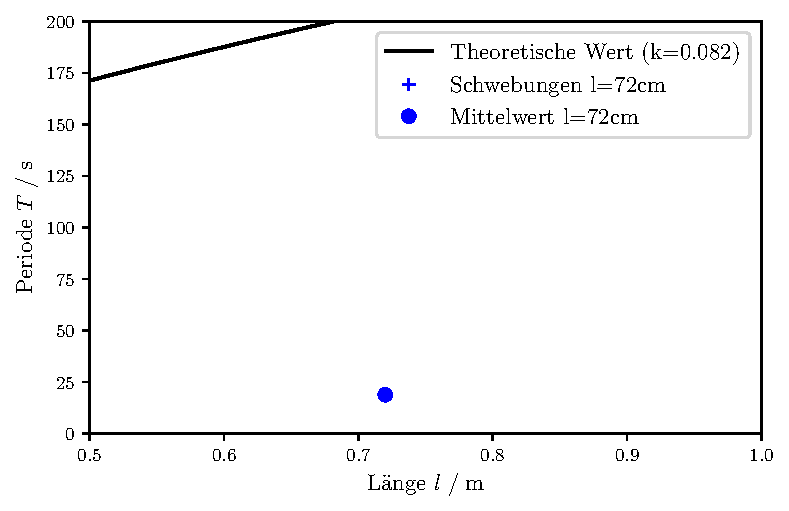
\includegraphics{build/plot6.pdf}
    \caption{Hall Spannung in Abhängigkeit vom Querstrom - Zink}
    \label{fig:Zn_B}
\end{figure}
Mit der Ausgleichsgeraden
\begin{align*}
    y &= mx + b\\
    m &= \SI{-391 \pm 3 e-02}{\volt \per \ampere}\\
    b &= \SI{2 \pm 1}{\volt}\\
\end{align*}
Aus der Steigung der Ausgleichsgeraden werden die mikroskopischen Parameter berechnet.
\begin{table}[H]
    \centering
    \begin{tabular}{c c}
        \toprule
        Größe & Wert\\
        \midrule
        $n$   &\SI[per-mode=fraction]{2,052\pm 0,017 e+27}{\per \cubic \metre}\\
        $z$   &\num{0,03121\pm 0,00025}\\
        $\bar{\tau}$ & \SI{5,76\pm 0,05 e-13}{\second}\\
        $\vec{\bar{v}}_d$ & \SI[per-mode=fraction]{0,003042\pm 0,000025}{\metre \per \second} \\
        $\mu$ & \SI[per-mode=fraction]{0,06}{\coulomb \second \per \kg}\\
        $v_{total}$ & \SI[per-mode=fraction]{4,551\pm 0,012 e+05}{\metre \per \second}\\
        $\bar{l}$ &\SI{2,624\pm 0,014 e-07}{\metre}\\
        \bottomrule
    \end{tabular}
    \caption{Hall Spannung für Kupfer- konstanter Duchflussstrom}
    \label{tab:Cu_B}
\end{table}


\subsubsection{Hall Spannung bei konstantem Querstrom}
% Data 5
\begin{table}[H]
    \centering
    \begin{tabular}{c c c}
        \toprule
        $I_{Spule} \;/\;$A & $U_H\;/\;$mV & $I_{durch} \;/\;$A\\
        \midrule
            0                   &-0,4094&             10\\
            0,5                 &-0,4042&             10\\
            1,0                 &-0,4024&             10\\
            1,5                 &-0,4004&             10\\
            2,0                 &-0,3981&             10\\
            2,5                 &-0,3981&             10\\
            3,0                 &-0,3950&             10\\
            3,5                 &-0,3928&             10\\
            4,0                 &-0,3900&             10\\
            4,5                 &-0,3880&             10\\
            5,0                 &-0,3800&             10\\
        \bottomrule
    \end{tabular}
    \caption{Hall Spannung für Zink- konstanter Durchflussstrom}
    \label{tab:Zn_B}
\end{table}
% Plot 5
\begin{figure}[H]
    \centering
    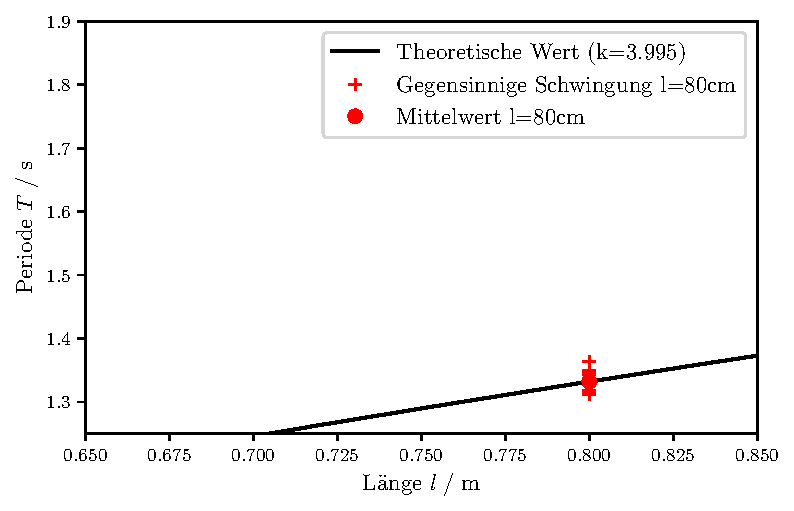
\includegraphics{build/plot5.pdf}
    \caption{Hall Spannung in Abhängigkeit vom Magnetfeld - Zink}
    \label{fig:Zn_B}
\end{figure}
Mit der Ausgleichsgeraden
\begin{align*}
    y &= mx + b\\
    m &= \SI{19 \pm 1}{\square \meter \per \second} \\
    b &= \SI{-409 \pm 1}{\volt} \\ 
\end{align*}
Mithilfe der Steigung $m$  wurden die mikroskopischen Parameter bestimmt.
\begin{table}[H]
    \centering
    \begin{tabular}{c c}
        \toprule
        Größe & Wert\\
        \midrule
        $n$   &\SI[per-mode=fraction]{3,23\pm 0,24 e+28}{\per \cubic \metre}\\
        $z$   &\num{0,49\pm 0,04}\\
        $\bar{\tau}$ & \SI{3,67\pm 0,28 e-14}{\second}\\
        $\vec{\bar{v}}_d$ & \SI[per-mode=fraction]{0,000194\pm 0,000015}{\metre \per \second} \\
        $\mu$ & \SI[per-mode=fraction]{0,06}{\coulomb \second \per \kg}\\
        $v_{total}$ & \SI[per-mode=fraction]{1,140\pm 0,029 e+06}{\metre \per \second}\\
        $\bar{l}$ &\SI{4,18\pm 0,21 e-08}{\metre}\\
        \bottomrule
    \end{tabular}
    \caption{Hall Spannung für Kupfer- konstanter Duchflussstrom}
    \label{tab:Cu_B}
\end{table}

\label{sec:Auswertung}
